%04chapterFremdeinsch.tex
\chapter{Gruppeneinschätzung des Teams}\label{Gruppenteameinschätzung}

Als Anregung unserer Diskussion zur Gruppeneinschätzung und damit wir einen Leitfaden haben, verwenden wir das Dokument Leitfragen für Team-Selbsteinschätzung (REFERENZ EINFÜGEN). Aus diesem Dokument haben wir folgende Fragen kopiert, welche wir nun beantworten werden.
  
\subsection*{Wie diskutieren die Teammitglieder Probleme?}

Die Mehrheit der Gruppe findet, dass die Probleme offen angesprochen werden. Jedoch findet Pascal, dass Probleme viel öfter zur Sprache gebracht werden und konstruktive Kritik an der Tagesordnung sein sollte. 
Probleme wurden Anfangs nur in Sitzungen angesprochen. Dies wollen wir ändern und zu einem laufenden Prozess machen. 

\subsection*{Wie gehen Teammitglieder mit Defiziten und unproduktiven Verhaltensweisen um?}

Anfangs waren die Arbeitszeiten sehr hoch. Dies wurde im Team schnell so zur Diskussion gebracht und Verbesserungsvorschläge unterbreitet. Nach einigen Diskussionen haben wir einiges an unserem Vorgehen angepasst und hoffen nun auf eine Effizienzsteigerung. Daher glauben wir, dass wir mit Defiziten und unproduktiven Verhaltensweisen sehr offen umgehen.

\subsection*{Was wissen Sie darüber, was Ihre Kollegen gerade machen und was Sie zum
Gruppenziel beitragen?}

Aufträge wurden jeweils am Anfang der Vorlesung jede Woche neu verteilt. In der Zwischenzeit war oft nicht klar, wer was bereits erledigt hat. Durch vermehrte Nutzung von MS-Project, erhöhtem Koordinationsaufwand (Aufträge in kürzeren Abständen) und einer klar definierten Führung, erhoffen wir uns mit weniger zeitlichem Aufwand bessere Produkte erstellen zu können.

\subsection*{Wie verhalten sich Teammitglieder, wenn sie etwas Unpassendes oder möglicherweise Teamschädliches gesagt oder getan haben?}

Keiner der Teammitglieder hatte bisher das Gefühl, teamschädigenden oder unpassenden Aussagen ausgesetzt zu sein.

\subsection*{Wie gehen Sie mit Wissensunterschieden im Team um?}

Das Wissen in unserem Team war und ist sehr unterschiedlich verteilt. 
In der Regel werden die Wissensunterschiede im Team gemeinsam ausgeglichen oder es wird erwartet, dass sich die Person selbstständig informiert. Als konkretes Beispiel ist zu erwähnen, dass am Anfang Gökhan bereits latex und Git Erfahrung hatte, während sich die anderen Teammitglieder noch nicht mit mit diesen Medien auseinandergesetzt hatten. Pascal und Gökhan haben sich selbstständig und ohne weitere Hilfe mit den neuen Medien auseinandersetzten, wobei dies bei Gerome teilweise nicht möglich war, da unter anderem ein entsprechend ausgestatteter Computer fehlte. Der dabei entstandene Wissensunterschied wird momentan in der Gruppe gemeinsam aufgeholt und gleichzeitig erwartet, dass sich Gerome selbstständig weiterbildet.  

\subsection*{Wie würden Sie Ihr Teamverhalten gegenüber Aussenstehenden (andere Abteilungen,
Kunden, Lieferanten) beschreiben?}

Der einzige Kontakt gegenüber Aussenstehenden ist der Dozent. Dieser ist zufriedenstellend. 

\subsection*{Wie zeigen Teammitglieder Engagement? Woran erkennen Sie (fehlendes)
Engagement?}

Das Teamengagement der Teammitglieder kann durch diverse Verhaltensweisen erkannt werden. Nachfolgend listen wir einige wichtige Erkennungsmerkmale auf.

\begin{itemize}

\item Freiwilliges Übernehmen von kleineren ausstehenden Arbeiten

\item Bereitschaft länger zu arbeiten, als dies zwingend nötig wäre

\item Beteiligung an Diskussionen

\item Pünktlichkeit

\end{itemize}

Bei Pascal ist zu erkennen, dass er oft kleinere anstehende Arbeiten freiwillig übernimmt und nicht zwingend notwendige arbeiten erledigt, damit das Projekt einem noch höheren Standard gerecht wird. 

Gökhan nimmt sich bei technischen Schwierigkeiten gerne für jeden Zeit und beteiligt sich ausserdem konstruktiv an Gesprächen.  

Gerome beteiligt sich ebenfalls gerne und konstruktiv an Gesprächen. Er hat eine ausserordentlichen Bereitschaft, längere Arbeitssessionen mit der Gruppe zu führen und dabei immer gut gelaunt zu bleiben. Die Pünktlichkeit lässt jedoch etwas zu wünschen übrig.  

\subsection*{Wie würden Sie Ihre Teamsitzungen beschreiben? Welchen Beitrag leisten diese zum
Teamerfolg?}

Der hauptsächliche Mehrwert, der in den bisherigen Sitzungen generiert wurde, war der Wissensausgleich der einzelnen Teammitglieder. Vor allem anfangs wurde aber noch zu wenige konkrete Handlungen aus diesen Sitzungen abgeleitet. 

\subsection*{Wie verhalten Sie sich, wenn Sie merken, dass die Gruppenziele (möglicherweise)
nicht erreicht werden können?}

Als wir den Gesammtumfang des AC-Produktes das erste mal vor Augen hatten, wurde uns bewusst, dass wir dieses nur mit einer neuen Strategie, bei welcher eine Person eine erhöhte koordinierende Rolle einnimmt bewältigt werden kann. 

\subsection*{Was wissen Sie über das Privatleben der anderen Teammitglieder?}

Während den gemeinsam erledigten Arbeiten konnten wir uns bereits privat etwas besser kennenlernen, indem wir beispielsweise gemeinsam gekocht haben, als wir längere Arbeiten verrichten mussten. 

\subsection*{Wie treffen Sie Entscheidungen im Team?}

Wie in unserem Regeldokument beschlossen, wurden Entscheidungen bisher nach dem Prinzip des Mehrheitsentscheides gefällt.

\subsection*{Was tun Sie, wenn Sie mit einer Entscheidung nicht einverstanden sind?}

Die Diskrepanz wird zur Sprache gebracht und anschliessend demokratisch entschieden.

\subsection*{Wie gehen Sie mit Lob und Kritik im Team um?}

Es wird versucht konstruktiv mit Kritik umzugehen. Der Kritiker hat sich bisher noch nie böswillig geäussert, so dass der kritisierte die Möglichkeit hatte, konstruktiv damit umzugehen. 

\subsection*{Welche Momente waren die schwierigsten im Team? An welche erinnern Sie sich
gerne?}

Die schwierigsten waren jene Momente, als wir bis spät abends unsere Freizeit für TKI eingesetzt hatten und schlussendlich doch nicht zufrieden sein konnte. 

Der beste Momente für unser Team war, als wir die gute Bewertung für das Teamreview 1 vom Dozenten bekamen.  

\subsection*{Wenn Sie erneut starten könnten, was würden Sie anders machen?}

Hätte sich unser Team immer frühzeitig über den anstehenden Auftrag informiert und Beispielprodukte vom Dozenten angefordert, hätte dies viel Klarheit geschafft und unsere Arbeitseffizienz gesteigert. Dies sind die Punkte, die wir anders machen würden. 

\subsection*{Resultat}

Nach langer Diskussion haben wir unser Team in den einzelnen Bereichen wie in Grafik (REFERENZ) ersichtlich eingeschätzt.

%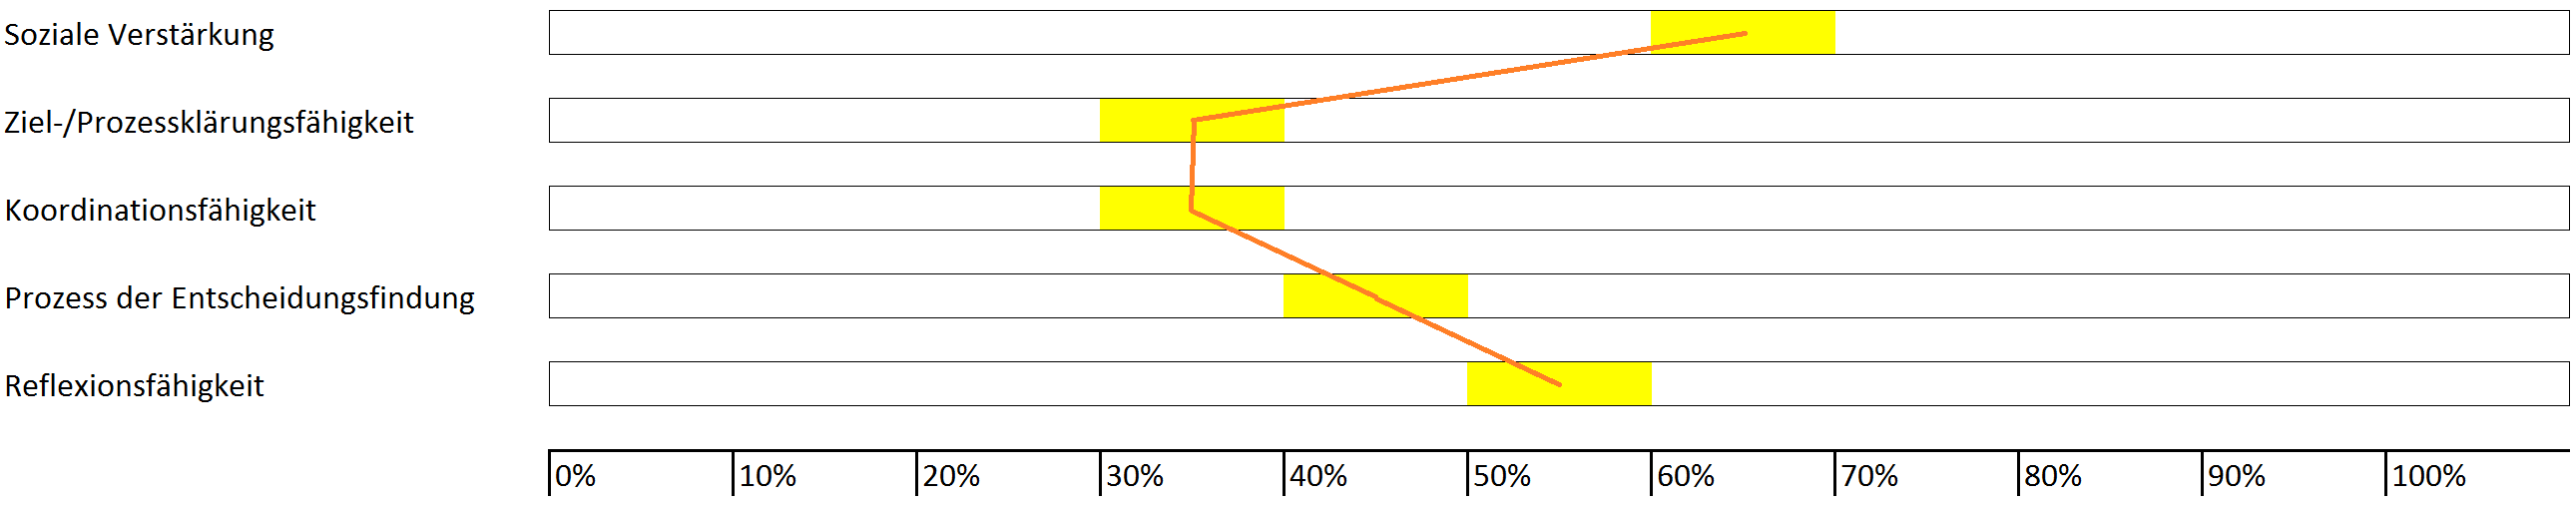
\includegraphics[height=10cm]{images/Gruppeneinsch.png}

Am wenigsten ausgeprägt sind die beiden Punkte Prozessklärungsfähigkeit und Koordinationsfähigkeit. Hier hat unser Team das grösste Verbesserungspotenzial. Der Punkt, der am besten bewertet wurde ist die Reflexionsfähigkeit und wir finden, dass wir unser Teamverhalten oft sehr genau analysieren können. 

\begin{comment}
Nach unseren individuell erstellten Selbsteinsch"atzungen, folgen nun die Fremdeinsch"atzungen, welche f"ur
den Vergleich von Selbst- und Fremdbild unabdingbar sind.
Dazu hat jedes Teammitglied seine eigene Form der Bearbeitung gew"ahlt. Dies war einerseits der Selbsteinsch"atzungstest, andererseits wurden anhand von spezifisch beobachteten Situationen eine Teamrollenzuteilung
vorgenommen.
\subsection*{Pascal Horat}

Auch um meine Teamkameraden einzuschätzen habe ich mich des vorher beschriebenen Belbin-Tests bedient. Dies vor allem aus drei Gründen:
\begin{enumerate}
\item Durch die vorgegebene Form ergibt sich meiner Meinung nach eine neutralere Betrachtung der Teamitglieder, da meine Einschätzung nicht nur auf ein bis zwei spezifischen Vorfällen beruht.
\item Durch die vorgegebene Form mit den Aussagen werde ich durch das Verfahren geleitet und muss nicht selber etwas entwickeln.
\item Da für die Bestimmung der Selbst- sowie der Fremdeinschätzung derselbe Test verwendet wurde, können direkte Vergleiche zwischen den Teammitgliedern gemacht werden.
\end{enumerate}

Dies hat für Gerome folgende Resultate hervorgebracht:



Von meinen Teammitgliedern fiel es mir, ohne die Hilfe des Tests, schwieriger, Gerome eine passende Rolle zuzuteilen. Darum hätte ich eine ausgeglichenere Punkteverteilung bei der Auswertung erwartet. Die Rolle des Ausgleichers, bei welcher er am meisten Punkte sammelte, finde ich jedoch passend. Dass sie bei ihm aber so ausgeprägt zum Zuge kommt, hat mich eher überrascht.

Bei Gökhan sieht die Auswertetabelle folgendermassen aus:



Bei ihm habe ich schon im Vornherein erwartet, dass er punktemässig eine Ausgleicher-Rolle erhalten würde. Interessanterweise war diese Rollenzuteilung aber viel ausgeglichener als vorher bei Gerome obwohl ich instinktiv eher das Gegenteil erwartet hätte. 

\subsection*{Steve Gerome Kamga}

Meine beiden Teammitglieder wurden auch von mir mit der Belbin-Methode eingeschätzt und die Ergebnissen werden folgendermassen dargestellt: \\
Nach meiner Einschätzung kam heraus, dass Pascal die nachfolgenden Rollen in einem Team übernehmen könnte:
\begin{enumerate}
\item Koordinator
\item Prozessgestalter
\item Bewerter
\end{enumerate}


Gökhan dagegen ist meiner Meinung nach mehr der:
\begin{enumerate}
\item Bewerter
\item Spezialist
\item Ausgleicher
\end{enumerate}


\subsection*{Gökhan Kaya}

Ich habe meine zwei Teamkollegen folgendermassen eingeschätzt:\\

Pascal war für mich der Koordinator und zwar aus den folgenden erlebten Gründen:
\begin{enumerate} 
\item{Meist sagt Pascal am Anfang der Sitzung was zu tun ist und gibt uns einen kleinen Überblick. Er ist somit sehr gut organisiert.}
\item{Er ist meistens der erste, der sich mit dem Dozenten in Verbindung setzt, wenn etwas noch unklar ist. Die nötigen Informationen leitet er uns anschliessend weiter.}
\item{Bereits bei der ersten Vorlesung ist mir aufgefallen, dass Pascal sich sehr vieles notiert und teilweise nach der Vorlesung ebenfalls mitteilt, was er sich notiert hat.}
\end{enumerate}

Gerome war für mich ganz klar der Vollender. Dies aus den folgenden drei Gründen:
\begin{enumerate} 
\item{Gleich nach der Teambildung konnte Gerome noch nicht auf moodle zugreifen. Er hat sich nach einem Tag bereits sofort gemeldet und mitgeteilt, dass bei ihm nun alles soweit funktioniert. Dies obwohl es nicht nötig gewesen wäre.}
\item{Ebenfalls hat nach der ersten Aufgabenteilung sofort auf WhatsApp geschrieben und uns mitgeteilt, dass er sein Auftrag erledigt hat. Pascal und ich empfanden dies hingegen als nicht nötig.}
\item{Als wir am letzten Tag vor der Abgabe noch bis spät die Lernbilanzen fertig gestellt haben, hat Gerome die ersten zwei Stunden ausschliesslich recherchiert, um das bestmögliche Produkt abzugeben. Dies obwohl wir nur wenig Zeit hatten. Dabei machte es ihm auch nichts aus, bis spät in die Nacht hinein zu arbeiten.}
\end{enumerate}

\end{comment}
